% -----------------------------*- LaTeX -*------------------------------
\documentclass[11pt]{report}
\usepackage{scribe_ds603}
\DeclareMathOperator*{\argmin}{arg\,min}
\begin{document}




\scribe{Nikhil Jha}		% required
\lecturenumber{10}			% required, must be a number
\lecturedate{26/09/2025}		% required, omit year


\maketitle


% ----------------------------------------------------------------------

\section{Defense Categories}
A survey paper on Security against Data-poisoning \cite{10.1145/3585385}, the current defenses against poisoning attacks can be classified in five categories:

\begin{enumerate}[label=\(\circ\), leftmargin=*, widest=b, align=left]
\item Training Data Sanitization: This defense involves elimination of poisoned or perturbed data samples through anomaly detection methods and obtaining a relatively cleaner dataset for training.

\item Loss Function modification: Loss function is modified such that the model remains robust against poisoned samples.

\item Model Inspection: Returns if the model has been compromise by an attack (Say for example, backdoor attacks).

\item Model Sanitization: Cleans the model to remove potential backdoors or targeted poisoning attempts.

\item Test Data Sanitization: Removes the test samples which might consider triggers for a backdoor attack.
\end{enumerate}

\section{Training Data Sanitization}

Data sanitization is mainly detecting anomalous samples and removing them from training dataset. Defenses differ in how they judge points as being anomalous\cite{10.1007/s10994-021-06119-y}. We represent each defense by a \textit{score function} \(s_{\beta}:\mathcal{X}\times\mathcal{Y} \rightarrow \mathbb{R}\) which takes a data-point and returns how anomalous it is. Following are different types of defenses with their score functions:

\begin{enumerate}[label=\textup{(\alph*)}, leftmargin=*, widest=b, align=left]
\item \label{mpp:gen_a_0} The L2 defense removes points far from class centroids in L2 distance:
\[\beta_y = \mathbb{E}_{\mathcal{D}}[x|y]\]
\[s_{\beta}(x,y) = ||x-\beta_y||_2\]
    
\item \label{mpp:gen_a_1}  The Slab defense projects points onto lines connecting centroids, and then removing points far from the centroids. Unlike L2 defense which treats all dimensions equally, slab only treats vector between class centroids as the relevant dimension.
\[\beta_y = \mathbb{E}_{\mathcal{D}}[x|y]\]
\[s_{\beta}(x,y) = |(\beta_1-\beta_{-1})(x-\beta_y)|\]


 \item \label{mpp:gen_a_2} Loss Defense discards points which are not well fit by the model.
 \[\beta = \argmin_{\theta}\mathbb{E}_{\mathcal{D}}[\ell_{\theta}(x,y)]\]
 \[s_{\beta}(x,y) = \ell_{\beta}(x,y)\]


 \item \label{mpp:gen_a_3} k-NN defense removes points that are far from their k-nearest neighbors.
 \[\beta = \mathcal{D}_c \cup \mathcal{D}_p\]
 \[s_{\beta}(x,y) = Distance\; to\; k^{th}\; nearest\; neighbor\]

 \item \label{mpp:gen_a_4} The SVD defense assumes that clean data lies in some low-rank subspace and hence poisoned must have large component outside of this subspace. If \(X\) is data matrix:
 \[\beta = [u_i]_{d\times m}\]
 \[s_{\beta}(x,y) = ||(I-\beta\beta^T)x||_2\]
 \[X=U\Sigma V^T, \;with\; U = [u_i]_{d\times r}\]

 \item \label{mpp:gen_a_5} Spectral Filtering is a more generalized defense of which SVD defense is a special case.
 \[s(x,y) = ||(\phi(x)-\hat{\phi})^Tv_j||_2\; where\; \phi:\mathbb{R}^d\rightarrow \mathbb{R}^k\]
 \[\hat{\phi} = \frac{1}{n}\sum_{i=1}^n\phi(x_i)\; and\; \Phi = U\Sigma V^T = [\phi(x_i)]_{i=1}^n \in \mathbb{R}^{n\times k}\]

 
 \end{enumerate}

\subsection*{Efficacy}
\begin{figure}[h!]
    \centering
    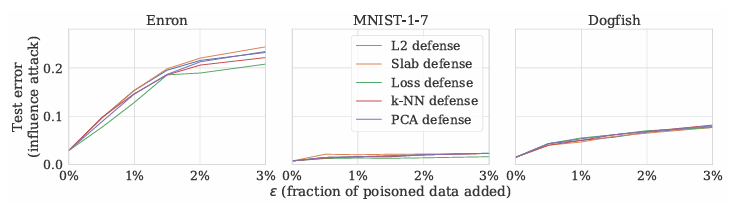
\includegraphics[width=0.8\linewidth]{images/data_sanit.png}
    \caption{The image taken from \cite[pg 42]{10.1007/s10994-021-06119-y} shows efficacy of different sanitization based defenses against Influence attack on Enron, MNIST 1-7 and Dogfish datasets.}
    \label{fig:placeholder}
\end{figure}

The influence attacks finds a poisoned data that maximizes loss for a fixed feasible set via projected gradient descent. As can be seen from the figure, the defenses work very well for MNIST 1-7 dataset and to some extent on Dogfish dataset as well. However, it does not seem to be that effective on Enron dataset. This might be due to MNIST 1-7 and Dogfish datasets being much easily linearly separable compared to Enron which makes anomaly detection easier.

\section{Loss Function Modification}

For this part, the threat model chosen is class-conditional noise model. The objective is to propose a modified loss function which is an unbiased estimator of true loss\cite{NIPS2013_3871bd64}. A class-conditional random noise model is given by:
\[P(\Tilde{Y} = -1| Y = +1) = \rho_{+1},\; P(\Tilde{Y}=+1|Y=-1)=\rho_{-1},\; and \rho_{+1}+\rho_{-1}<1\]

\noindent It is assumed that the noise rates are known. \\ Let \(L=\mathbb{E}_{(x,y)\sim\mathbb{P}^*}[\ell(z,h)],\; \hat{L}=\frac{1}{n}\sum_{i=1}^n\ell(z_i,h),\; \Tilde{L}=\mathbb{E}_{(x,\Tilde{y})\sim\Bar{\mathbb{P}}}[\Tilde{\ell}((x,\Tilde{y}),h)],\; \hat{\Tilde{L}}=\frac{1}{n}\sum_{i=1}^n\Tilde{\ell}((x_i,\Tilde{y}_i),h)\). \(\Bar{\mathbb{P}}\) is the distribution of \((x,\Tilde{y})\).

\noindent Let \(\hat{\Tilde{h}} \in \argmin_{h\in \mathcal{H}}\hat{\Tilde{L}}(h)\) and \(\ell\) is \(\beta\)-lipschitz in \(h(x)\) with \(h:\mathcal{X}\rightarrow \mathbb{R}\) and bounded.

\begin{lemma}
    If \[\Tilde{\ell}(t,y) \Let \frac{(1-\rho_{-y})\ell(t,y)-\rho_y\ell(t,-y)}{1-\rho_{+1}-\rho_{-1}}\]
    then \(\mathbb{E}_{\Tilde{y}}[\Tilde{\ell}(h(x),\Tilde{y})]=\ell(h(x),y)\).
\end{lemma}

\begin{proof}
    We want for every \(t\), \(\mathbb{E}_{\Tilde{y}}[\Tilde{\ell}(t,y)] = \ell(t,y)\). Then considering cases for \(y=+1\; and \; y=-1\) separately
    \[(1-\rho_{+1})\Tilde{\ell}(t,+1)+\rho_{+1}\Tilde{\ell}(t,-1)=\ell(t,+1)\]
    \[(1-\rho_{-1})\Tilde{\ell}(t,-1)+\rho_{-1}\Tilde{\ell}(t,+1)=\ell(t,-1)\]

    Solving the two equations give the expression in lemma above.
\end{proof}

\begin{lemma}
    \[\sup_{h \in \mathcal{H}}|\hat{\Tilde{L}}(h)-\Tilde{L}(h)|\leq 2\beta_{\rho}.Complexity(\mathcal{H})+\sqrt{\frac{log(1/\delta)}{2n}}\]
    where \(\beta_{\rho}\leq \frac{2\beta}{1-\rho_{+1}-\rho_{-1}}\) is the Lipschitz constant of \(\Tilde{\ell}\)
\end{lemma}

\begin{proof}
    Proof is to be done by Rademacher bound to be discussed later in class.
\end{proof}

\begin{theorem}\label{ThmNeat}
    \[L(\hat{\Tilde{h}})\leq L(h^*)+4\beta_{\rho}Complexity(\mathcal{H})+2\sqrt{\frac{log(1/\delta)}{2n}}\]
\end{theorem}

\begin{proof}
    By Lemma 1,
    \[\Tilde{L}(h) = L(h)\]
    hence,
    \[L(\hat{\Tilde{h}})-L(h^*) = \Tilde{L}(\hat{\Tilde{h}})-\Tilde{L}(h^*)\]
    i.e.,
    \[L(\hat{\Tilde{h}})-L(h^*) = (\Tilde{L}(\hat{\Tilde{h}})-\hat{\Tilde{L}}(\hat{\Tilde{h}}))+(\hat{\Tilde{L}}(\hat{\Tilde{h}})-\hat{\Tilde{L}}(h^*))(\hat{\Tilde{L}}(h^*)-\Tilde{L}(h^*))\]
    \[L(\hat{\Tilde{h}})-L(h^*) \leq 2\max_{h\in \mathcal{H}}|\hat{\Tilde{L}}(h)-\Tilde{L}(h)|\]
    substituting from lemma 2 we arrive at the expression in the theorem.
\end{proof}

\subsection*{Efficacy}
This method of loss function modification shows good results when tested on perfectly linearly separable dataset and non-separable banana dataset.
\begin{figure}[h!]
    \centering
    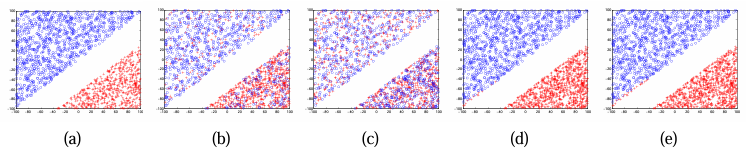
\includegraphics[width=\linewidth]{images/loss_mod1.png}
    \caption{ Classification of linearly separable synthetic dataset using \(\Tilde{\ell}_{log}\). The noise-free data is shown in the leftmost panel. Plots (b) and (c) show training data corrupted with noise rates(\(\rho_{+1}=
 \rho_{-1}=\rho\)) 0.2 and 0.4 respectively.  Plots (d) and (e) show the corresponding classification results. The algorithm achieves 98.5\% accuracy even at 0.4 noise rate per class.}
    \label{fig:placeholder}
\end{figure}

\begin{figure}[h!]
    \centering
    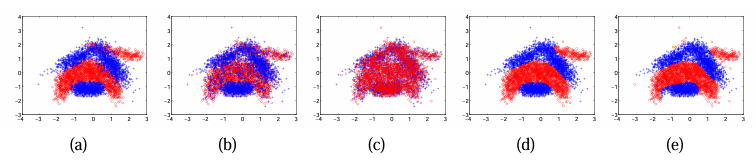
\includegraphics[width=\linewidth]{images/loss_mod2.png}
    \caption{Noise free data in (a). (b) and (c) shhow training data corrupted with noise rates 0.2 and 0.4 respectively. (d) and (e) show corresponding classification results. The accuracies are 90.8\% and 88.5\% respectively.}
    \label{fig:placeholder}
\end{figure}

\section{Model Inspection}

\begin{figure}[h!]
    \centering
    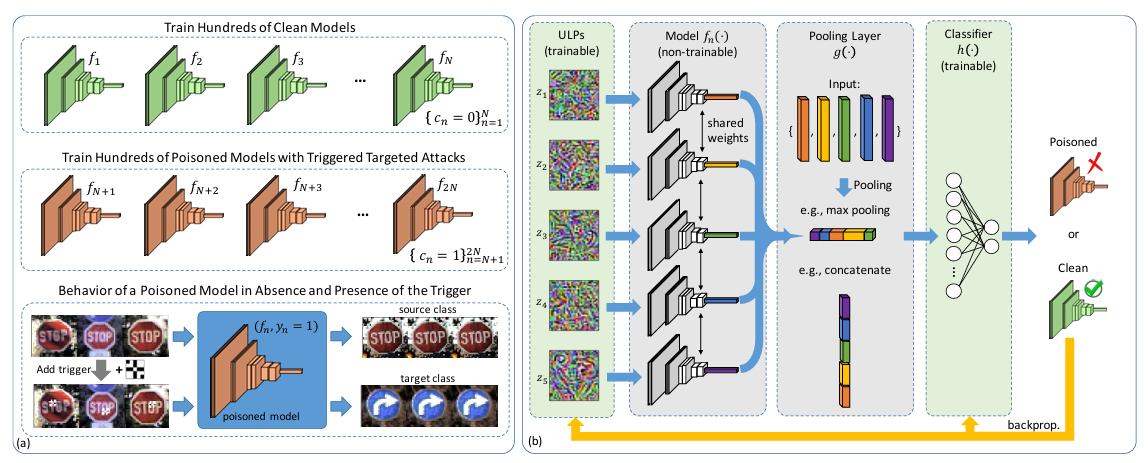
\includegraphics[width=0.9\linewidth]{images/ULP.png}
    \caption{Training a neural network to classify a model as clean or poisoned through ULPs}
    \label{fig:placeholder}
\end{figure}

It is a common practices to use pre-trained models as a part of some larger model as it saves a lot if time. Since pre-trained models are very often from third, potentially unknown party, there integrity cannot be guaranteed. If such models are trained to misclassify by backdoor triggers, they might look completely normal on clean training dataset.

Universal Litmus Patterns(ULPs)\cite{9157782} offer a method to classify a model as clean or poisoned. The idea is to train a classifier and its input(these inputs are called ULPs). Note that the framework as given in Figure 11.4(b) is not classifying an image but the neural network shown as untrainable part in the diagram. The optimization is
\[\argmin_{z,h} \sum_{n=1}^N L(h(g({f_n(z_m)}_{m=1}^M)),c_n)+\lambda\sum_{m=1}^M R(z_m)\]
\noindent where \(f_n(z_m)\) denotes the logit output by classifier \(f_n\) for ULP \(z_m\), \(h\) is the classifier that receives pooled vector from as inputs and gives probability of \(f_n\) being poisoned or clean, \(c_n\) is the actual label for \(f_n\).

\subsection*{Results}
\begin{figure}[h!]
    \centering
    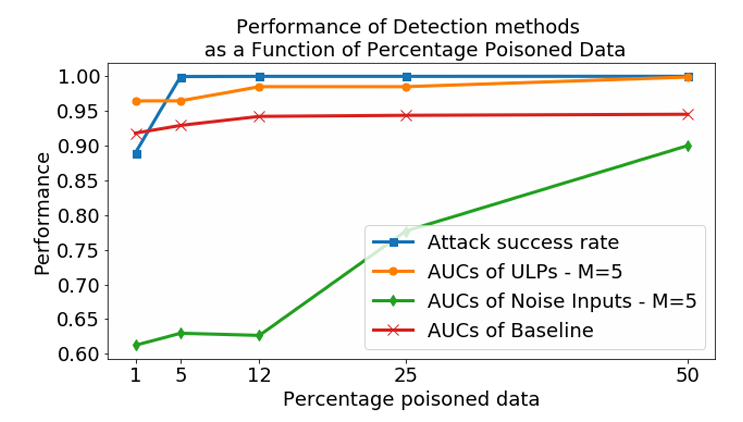
\includegraphics[width=0.6\linewidth]{images/ULP_res.png}
    \caption{Performance of ULPs as a function of poisoned to clean ratio. The test set consisted of 900 models(450 from each class), and the training set contained 900 models(each trained with 50\% poisoned data)}
    \label{fig:placeholder}
\end{figure}

\section{Model Sanitization}

\subsection{Neural Attention Distillation}

Standard finetuning is often used to  erase backdoors, however, this methods seems to be more effective. Suppose, we have an outsourced pre-trained backdoored model. Lets call this model as student. The, we apply finetuning on this model to obtain another model and call it teacher. The student and teacher are then combined through Neural Attention Distillation process\cite{li2021neural}. This process is then carried out iteratively to finally obtain a clean model.

\textbf{Attention Representation: }Suppose \(F^l \in \mathbb{R}^{C\times H\times W}\) denote activation output at the l-th layer. Then we define an attention operator to map 3D activation to flattened 2D tensor. Following are the three possible formulations
\[\mathcal{A}_{sum}(F^l)=\sum_{i=1}^C |F^l_i|; \;\;\;\mathcal{A}^p_{sum}(F^l)=\sum_{i=1}^C |F^l_i|^p; \;\;\; \mathcal{A}^p_{mean}(F^l)=\frac{1}{C}\sum_{i=1}^C |F^l_i|^p\]

\noindent If we define attention distillation loss as

\[L_{NAD}(F_T^l, F_S^l) = \left\lvert\left\lvert\frac{\mathcal{A}(F_T^l)}{||\mathcal{A}(F_T^l)||_2} - \frac{\mathcal{A}(F_S^l)}{||\mathcal{A}(F_S^l)||_2}\right\rvert\right\rvert_2\]

\noindent The final loss function is then represent by
\[L_{total} = \mathbb{E}_{(x,y)\sim \mathcal{D}}[L_{CE}(F_s(x),y)+\beta . \sum_{l=1}^{K} L_{NAD}(F_T^l(x), F_S^l(x))]\]

\subsection{Implicit Backdoor Adversarial Unlearning}

\begin{algorithm2e}[!ht]
\DontPrintSemicolon
\SetKwInOut{ini}{Initialize}
\SetKwInOut{giv}{Data}
\SetKwInOut{out}{Output}
\giv{\(\theta_1\)(poisoned model);   D(clean set accessible for backdoor unlearning);}
\ini{\(C_{\delta}\)(\(l_2\) norm bound); K,T; \(\alpha, \beta\)}
i=1;\\
\While{\(i \leq K-1\)}
    {
    \(\delta_i \leftarrow \bold{0}^{1\times d}\); \\
     t = 1;\\
     \While{\(t\leq T\)}
     {
     Update \(\delta_i^{t+1} = \delta_i^{t}+\alpha \nabla_1 H(\delta_i^t(\theta_i), \theta_i)\);\\
     \delta_i = \delta_i \times min (1, C_{\delta}/||\delta_i||_2);\\
     t = t+1; \\
     }
    Compute \(\nabla{\delta_i^T}\) (Hessian products) via an iterative solver with reverse mode differentiation;\\
    \(\nabla_{\theta} \Tilde{\psi}(\theta_i) = \nabla_2 H(\delta_i, \theta_i)+\nabla \delta_i^T \nabla_1 H(\delta_i, \theta_i) \);\\
    Update \(\theta_{i+1} = \theta_i-\beta \nabla \Tilde{\psi}(\theta_i)\);\\
    i = i+1;\\
    }
  \out{\(\theta_K\)}  
\caption{I-BAU}
\label{alg:some_algo}
\end{algorithm2e}

This method\cite{zeng2022adversarialunlearningbackdoorsimplicit} first performs gradient ascent for finding perturbation that maximizes the empirical loss within bounds. Then,  gradient of this maxima to perform gradient descent on the model minimizing the perturbation that is most damaging hopefully obtaining a clean model in the process.

\begin{figure}[h!]
    \centering
    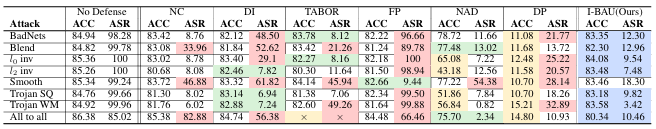
\includegraphics[width=\linewidth]{images/ibau.png}
    \caption{Results on CIFAR-10, one-trigger cases. The ASR against I-BAU is much lesser compared to other defenses with similar ACC.}
    \label{fig:placeholder}
\end{figure}

\section{Forensics}

\begin{figure}[h!]
    \centering
    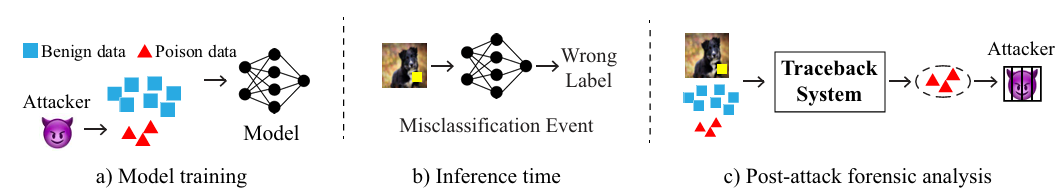
\includegraphics[width=\linewidth]{images/forensics.png}
    \caption{The general scenario for trackbask system. (a) the attacker poisons training data to inject vulnerability into the model; (b) attacker submits attack input to cause misclassification during run-time; (c) trackback system inspects the misclassification event to identify its root cause.}
    \label{fig:placeholder}
\end{figure}

\subsection{Intuition}
A high level overview of the trackback system\cite{281308} can be given as follows.

\textbf{Clustering unmarked training data.} The clustering component divides data into clusters based on how they affect model parameters based on the gradient given as \(\nabla_{\theta}\ell(\mathcal{F}(x), Uniform)\).

\textbf{Identifying and pruning innocent clusters. }The pruning component then examines unmarked clusters to remove less responsible clusters by comparing the losses on dataset trained with and without the cluster. If the loss without cluster is greater, it means cluster is responsible for misclassification.

\begin{figure}[h!]
    \centering
    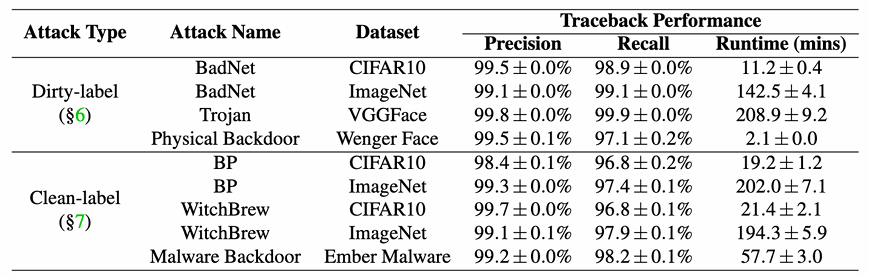
\includegraphics[width=\linewidth]{images/Forensics_ex.png}
    \caption{Precision, recall and runtime of the trackback system against dirty-label and clean-label poisoning attacks.}
    \label{fig:placeholder}
\end{figure}

\noindent\textbf{NOTE: The defense methods discussed so far do not consider attacks that are defense -aware and can adapt to the given defenses. For example, KKT and Min-max attacks have higher success rate compared to Influence attacks.}

\newpage

\section{Real-world Case Study of Art Generation: Are generative models resistant to poisoning attacks?}

Recently, using AI for imitating art of various artists has been on a rise.

\begin{figure}[h!]
    \centering
    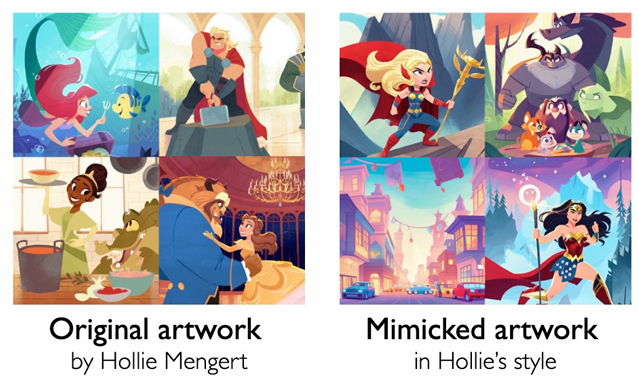
\includegraphics[width=0.7\linewidth]{images/art_mimic.png}
    \caption{Real-world incident of AI plagiarizing the style of artist Hollie Mengert}
    \label{fig:placeholder}
\end{figure}

\begin{figure}[h!]
    \centering
    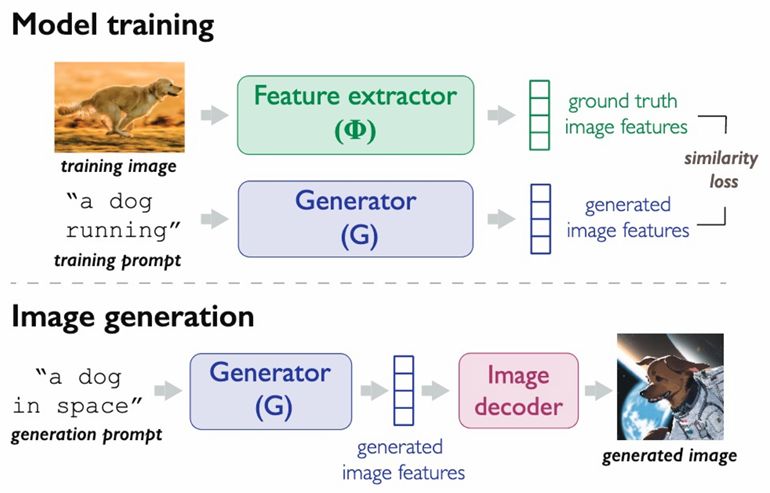
\includegraphics[width=0.7\linewidth]{images/text2img.png}
    \caption{High-level model architecture of text-to image models}
    \label{fig:placeholder}
\end{figure}

\noindent When artist post their artwork online, it is scraped and used to fine-tune pre-trained text-to-image models. This results in style-specific models which can mimic the victim artist's art-style. As such artworks are often directly scraped from websites, it is difficult to put a stop to such actions.

\subsection{Can imperceptible noise be added to the artworks resulting in poisoned dataset difficult for training?}

\textbf{Glaze} is a software built by Shawn Shan which is meant to help artists fight against plagiarism by AI. For a high-level intuition one can think of it taking and image and performing a style-transfer where the art-style of paining is changed which will then be used as a cloak. Glaze optimizes cloak for original artwork which makes the cloaked artwork similar to original in input space but more similar to the target cloak in \(\Phi\)'s feature space. Which means to a human eye, the cloaked work looks the same as original work but when a model is trained on this data, it would return art-style similar to the target artwork.

\begin{figure}[h!]
    \centering
    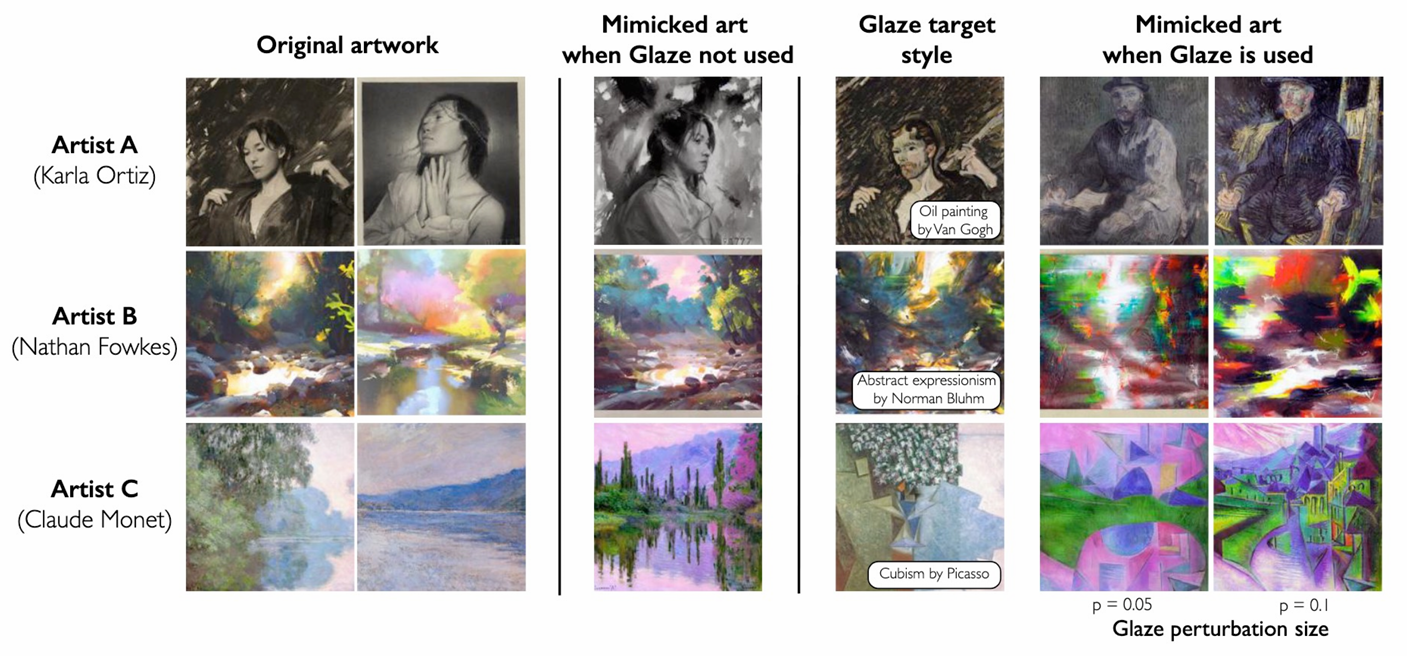
\includegraphics[width=0.8\linewidth]{images/glaze.png}
    \caption{Comparison of artworks without using glaze v/s when glaze is used.}
    \label{fig:placeholder}
\end{figure}

Even though Glaze seems to be very effective in this case, it still has its shortcomings. First, its not very useful for artists who have already posted their work online without using it. Hence, its of no use to older artists. Second, it is possible to build models robust to such perturbations which means that it might not be very relevant in the long run.

\begin{figure}[h!]
    \centering
    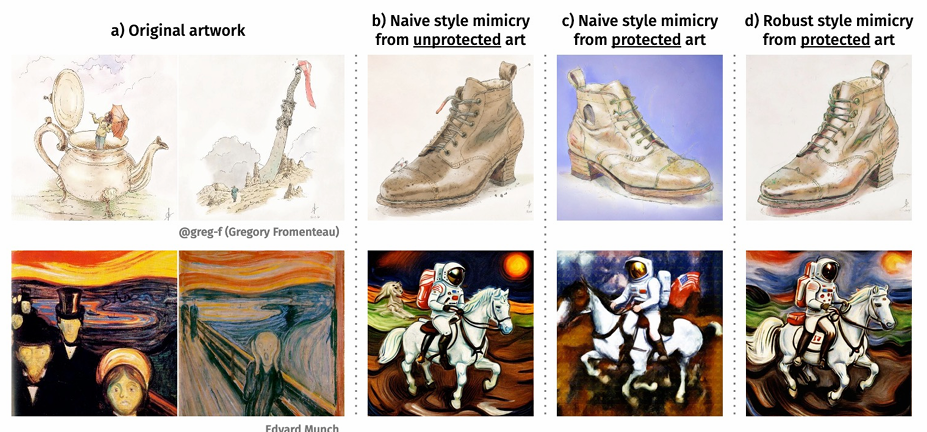
\includegraphics[width=0.7\linewidth]{images/robust.png}
    \caption{Examples of Robust style mimicry}
    \label{fig:placeholder}
\end{figure}

% Optional, if you want to make a comment about vulnerability of any result or so on.
%\begin{danger}
%This is the danger environment.
%\end{danger}


\bibliographystyle{plain}
\bibliography{refs}


\end{document}